%\documentclass[
%  paper=a4,
%  fontsize=11pt,
%  DIV=12,
%  parskip=half,
%  headings=normal
%]{scrartcl}
%
%\usepackage[ngerman]{babel}
%\usepackage{csquotes}
%\usepackage{microtype}
%\usepackage{booktabs}
%\usepackage{tikz}
%\usepackage{pgfplots}
%\pgfplotsset{
%  compat=1.18,
%  every axis/.append style={
%    font=\small,
%  },
%}
%\usepackage[firafull]{addfonts}
%\usepackage[hidelinks]{hyperref}

\documentclass{bfarticle}

\title{Künstliche Intelligenz\\eine Einführung}
\author{Benno Falkner}
\date{\today}

\begin{document}

\maketitle
\tableofcontents

\section{Einleitung}

Künstliche Intelligenz ist kein monolithisches Konzept, sondern ein Spektrum
von Methoden, Modellen und Paradigmen. Was heute unter dem Begriff subsumiert
wird, reicht von einfachen Klassifikationsalgorithmen bis zu großen
Sprachmodellen mit mehreren hundert Milliarden Parametern. Dieser Artikel
gibt einen strukturierten Überblick über die wichtigsten Konzepte.

\section{Grundlegende Konzepte}

\subsection{Maschinelles Lernen}

Maschinelles Lernen bezeichnet den Prozess, bei dem ein System aus Daten
lernt, ohne explizit programmiert zu werden. Der Kern ist die Optimierung
einer Verlustfunktion $\mathcal{L}$:

\[
  \mathcal{L}(\theta) = \frac{1}{N} \sum_{i=1}^{N} \ell(f_\theta(x_i), y_i)
\]

wobei $f_\theta$ das Modell mit Parametern $\theta$, $x_i$ die Eingabe und
$y_i$ die erwartete Ausgabe bezeichnen.

\subsection{Neuronale Netze}

Ein neuronales Netz besteht aus Schichten von Neuronen. Jede Schicht
transformiert ihre Eingabe durch eine gewichtete Summe und eine
Aktivierungsfunktion $\sigma$:

\[
  z^{(l)} = \sigma\!\left(W^{(l)} z^{(l-1)} + b^{(l)}\right)
\]

Die Wahl der Aktivierungsfunktion beeinflusst das Lernverhalten erheblich.
Tabelle~\ref{tab:aktivierung} gibt einen Überblick über gebräuchliche
Funktionen.

\begin{table}[h]
\centering
\caption{Gebräuchliche Aktivierungsfunktionen}
\label{tab:aktivierung}
\begin{tabular}{lll}
\toprule
Funktion & Definition & Wertebereich \\
\midrule
ReLU     & $\max(0, x)$                        & $[0, \infty)$ \\
Sigmoid  & $\frac{1}{1+e^{-x}}$               & $(0, 1)$ \\
Tanh     & $\frac{e^x - e^{-x}}{e^x + e^{-x}}$ & $(-1, 1)$ \\
Softmax  & $\frac{e^{x_i}}{\sum_j e^{x_j}}$   & $(0, 1)$ \\
\bottomrule
\end{tabular}
\end{table}

\subsection{Aktivierungsfunktionen im Vergleich}

\begin{figure}[h]
\centering
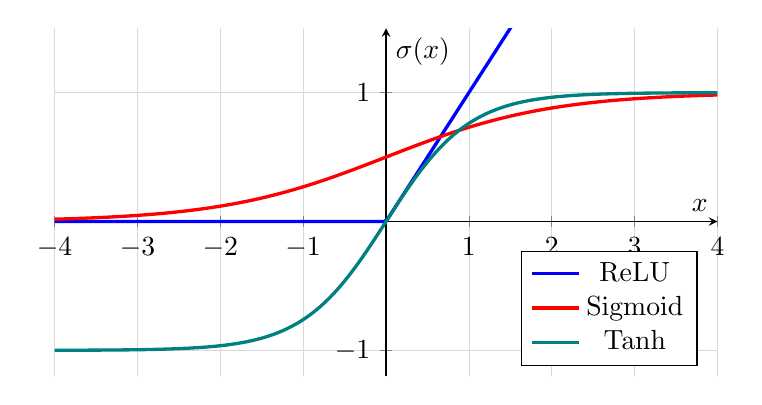
\begin{tikzpicture}
\begin{axis}[
  width=10cm,
  height=6cm,
  xlabel={$x$},
  ylabel={$\sigma(x)$},
  axis lines=center,
  xmin=-4, xmax=4,
  ymin=-1.2, ymax=1.5,
  grid=major,
  grid style={line width=0.2pt, draw=gray!30},
  legend pos=south east,
  every axis plot/.append style={line width=1.2pt},
]
\addplot[blue, domain=-4:4, samples=200] {max(0,x)};
\addlegendentry{ReLU}
\addplot[red, domain=-4:4, samples=200] {1/(1+exp(-x))};
\addlegendentry{Sigmoid}
\addplot[teal, domain=-4:4, samples=200] {tanh(x)};
\addlegendentry{Tanh}
\end{axis}
\end{tikzpicture}
\caption{Vergleich gebräuchlicher Aktivierungsfunktionen}
\end{figure}

\section{Große Sprachmodelle}

Große Sprachmodelle wie GPT oder Claude basieren auf der
Transformer-Architektur. Der zentrale Mechanismus ist die
\emph{Selbstaufmerksamkeit} (Self-Attention):

\[
  \text{Attention}(Q, K, V) = \text{softmax}\!\left(
    \frac{QK^T}{\sqrt{d_k}}
  \right) V
\]

wobei $Q$, $K$ und $V$ die Query-, Key- und Value-Matrizen bezeichnen und
$d_k$ die Dimension des Key-Vektors ist.

\section{KI im Bildungskontext}

Der Einsatz von KI in Schulen wirft grundlegende Fragen auf: Welche
Kompetenzen sollen Schülerinnen und Schüler erwerben? Wie verändert sich
die Rolle der Lehrperson? Und wie lässt sich sicherstellen, dass KI-Systeme
pädagogisch sinnvoll eingesetzt werden?

Ein sokratischer Ansatz — bei dem KI nicht Antworten liefert, sondern
Fragen stellt — könnte hier produktiver sein als reine Informationsvermittlung.

\section{Fazit}

KI ist kein Werkzeug das man versteht indem man es benutzt. Das Verständnis
der mathematischen Grundlagen, der Architekturentscheidungen und der
gesellschaftlichen Implikationen ist Voraussetzung für einen kompetenten
Umgang. Dieser Artikel hat einen ersten Einstieg gegeben — die Tiefe liegt
in den Details.

\end{document}